\section{Notable Circles}
\label{sec:09-inversion-circles}

Dozens of circles can be visualized with respect to the triangle family selected in \cref{sec:09-triangle-type}. These are selected via the (left) drop-down menu highlighted in \cref{fig:09-menu-circles}. The \texttt{circs off} setting is the default. The possible choices are organized in two groups: (i) ellipse-affixed, and (ii) central circles.

\begin{figure}
    \centering
    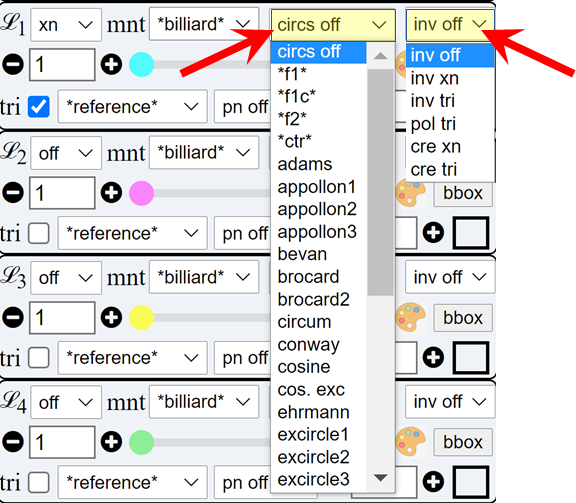
\includegraphics[width=.6\textwidth]{chap_09/pics/pics_09_100_circles_inv.png}
    \caption{The left drop-down selects an ellipse-based circle or a ``central'' circle for both visualization and/or as references for inversive transformations.}
    \label{fig:09-menu-circles}
\end{figure}

\subsection{Ellipse-Affixed Circles}

These are asterisk-decorated to indicate that they refer to a unit circle centered on a notable point of the ellipse (or caustic) used to generate a given triangle family, to be sure:

\begin{itemize}
\item \texttt{*f1*}: the left focus of the outer ellipse. Note: in the poristic (resp. excentral) family this becomes the center of the outer circle (resp. caustic = elliptic billiard).
\item \texttt{*f1c*}: the left focus of the inner ellipse. 
\item \texttt{*f2*}: the right focus of the outer ellipse. Note: in the poristic (resp. excentral) family this becomes the incenter (resp. a focus of the outer ellipse.
\item \texttt{*ctr*}: the center of the system.
\end{itemize}

\subsection{Central Circles}

Most of these are defined in \cite[Central Circles]{mw}:

\begin{itemize}
\item \texttt{adams}: the Adams circle
\item \texttt{appollon1,appollon2,appollon3}: 1st, 2nd, and 3rd Appollonius circles (which intersect on the isodynamic points)
\item \texttt{bevan}: the Bevan circle, circumcircle of the excentral triangle
\item \texttt{brocard,brocard2}: the Brocard circle and the so-called ``2nd'' Brocard circle.
\item \texttt{circum}: the circumcircle
\item \texttt{conway}: Conway's circle
\item \texttt{cosine}: the cosine (or 2nd Lemoine) circle 
\item \texttt{cos.exc}: the cosine circle of the excentral triangle
\item \texttt{ehrmann}: Ehrmann's 3rd Lemoine circle, see \cite{darij2012-ehrmann}.
\item \texttt{excircle1,excircle2,excircle3}: the three excircles
\item \texttt{euler}: Euler's circle
\item \texttt{furhmann}: Furhmann's circle
\item \texttt{gallatly}: Gallatly's circle
\item \texttt{gheorghe}: Gheorghe's circle, see \cite[X(649)]{etc}
\item \texttt{incircle}: Incircle
\item \texttt{lemoine}: 1st Lemoine circle
\item \texttt{lester}: Lester's circle
\item \texttt{mandart}: Mandart's circle
\item \texttt{moses,moses rad}: Moses's circle and Moses' radical circle
\item \texttt{parry}: Parry's circle
\item \texttt{reflection}: the ``reflection'' circle (circumcircle of the reflection triangle)
\item \texttt{schoutte}: Schoutte's circle
\item \texttt{spieker}: Spieker's circle
\item \texttt{taylor}: Taylor's circle
\end{itemize}

As shown in \cref{fig:09-three-circles}, several circles can be shown simultaneously. To do this select one for each channel (maintaining the same triangle family and type), and make sure to check the 

\begin{figure}
    \centering
    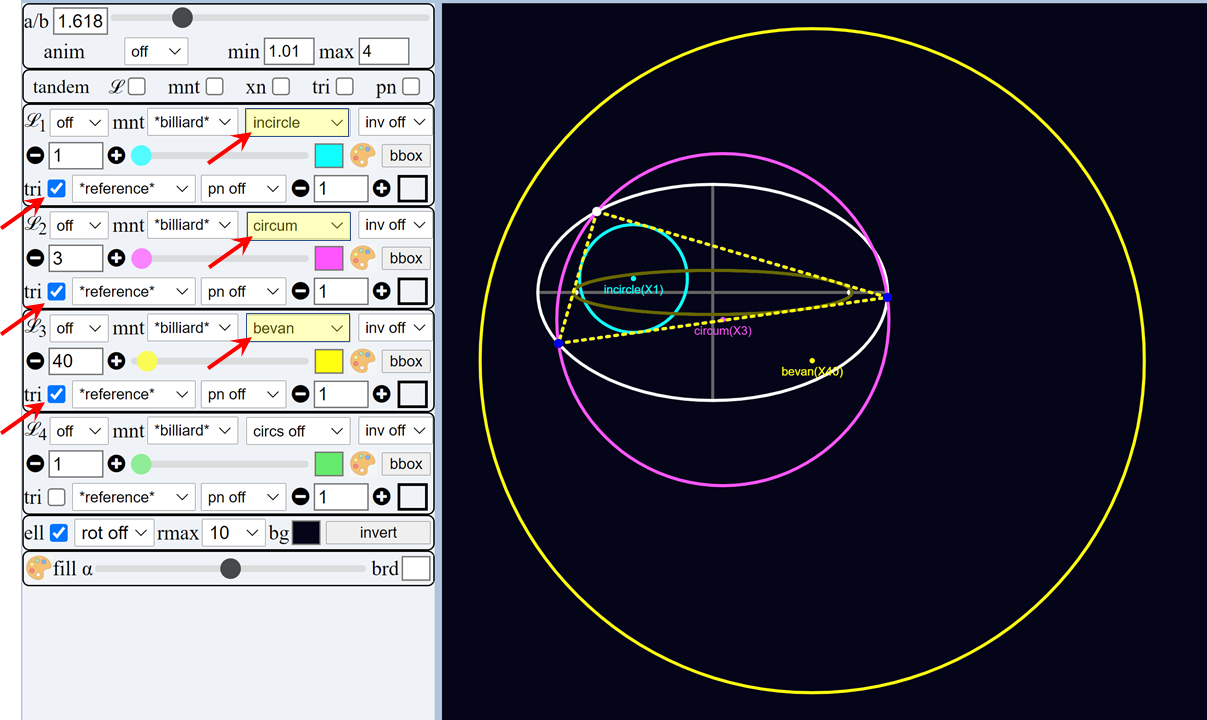
\includegraphics[width=.8\textwidth]{pics_09_110_simult_circs.png}
    \caption{The incircle, circumcircle, and Bevan circle are viewer simultaneously, by choosing them on the circle menu in 3 separate channels. Notice that to make the circle appear, one must check the \texttt{tri} checkbox in the lower left of that channel control area. \href{https://bit.ly/3poF5YQ}{Live}}
    \label{fig:09-three-circles}
\end{figure}

\section{Inversive Transformations with respect to a Circle}

Provided a circle $\Cm$ is selected (see above section), one can add an inversive-type transformation with respect to it. This is done via the (right) drop-down menu highlighted in \cref{fig:09-menu-circles}. The possible transformations are as follows: 

\begin{itemize}
    \item \texttt{inv off}: No transformation is performed.
    \item \texttt{inv xn}: invert the selected triangle center (see \cref{sec:09-triangle-center}) with respect to $\Cm$.
    \item \texttt{inv tri}: invert the vertices of triangles in the family with respect to $\Cm$.
    \item \texttt{pol tri}: compute a new triangle bounded by the polars of the original vertices with respect to $\Cm$.
    \item \texttt{cre xn}: send the selected triangle center to its image under a quadratic Cremona transformation (QCT) $(x,y)\rightarrow(1/x,1/y)$, where $(x,y)$ are the coordinated of the center of $\Cm$. 
    \item \texttt{cre tri}: compute a new triangle whose vertices are images of the QCT with respect to the center of $\Cm$.
\end{itemize}
